\documentclass[12pt, fleqn]{article}
% Преамбула

\usepackage[utf8]{inputenc}
\usepackage[T2A]{fontenc}
\usepackage[english,russian]{babel}
\usepackage{amssymb}
\usepackage[fleqn]{amsmath}
\usepackage{multicol}
\usepackage{array,graphicx,caption}
\usepackage{hyperref}
\usepackage[procnames]{listings}
\usepackage{color}
\usepackage{amsfonts} 
\usepackage{enumitem}
\usepackage{wrapfig}
\usepackage{cmap}

\begin{document}
\thispagestyle{empty}
\begin{center}
\ \vspace{-3cm}
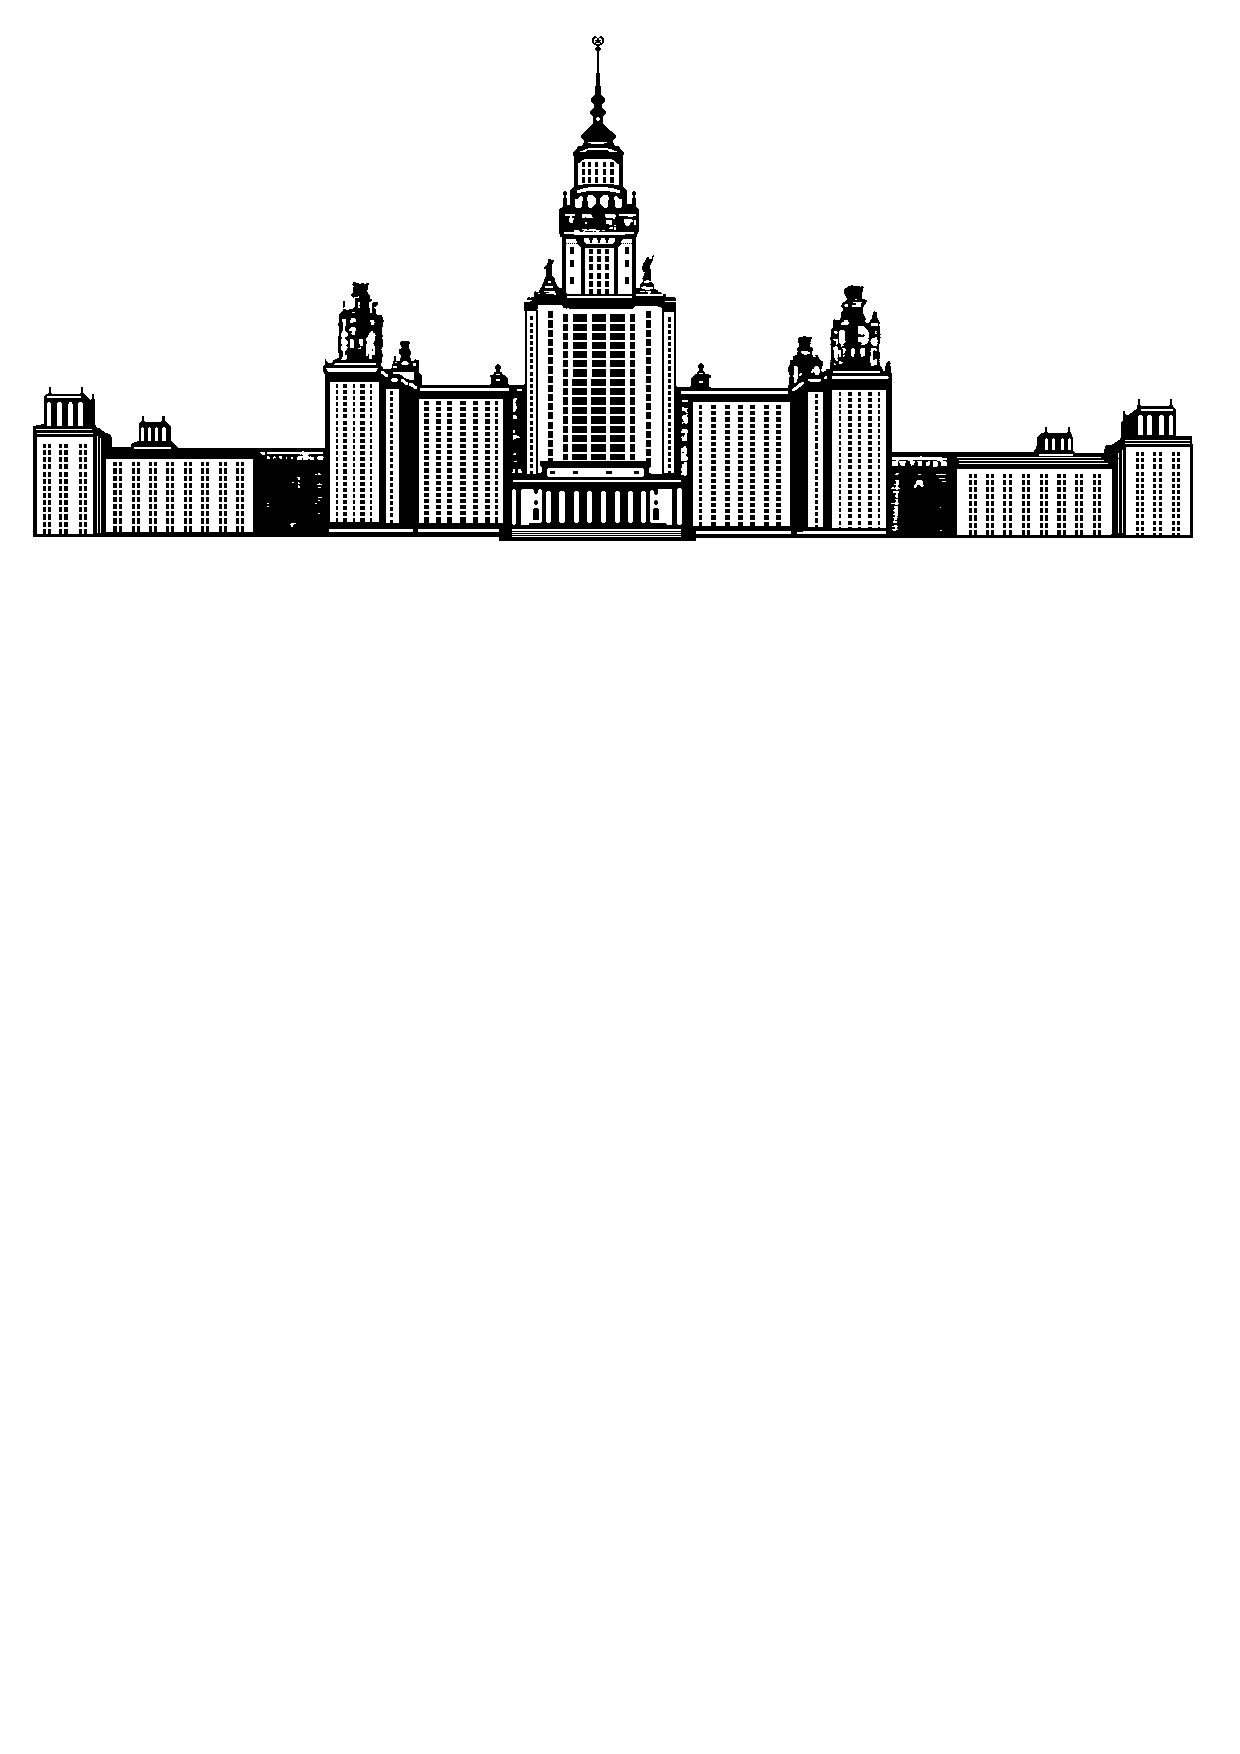
\includegraphics[width=0.3\textwidth]{i1.pdf}\\
{\scshape Московский государственный университет имени М.~В.~Ломоносова}\\
Факультет вычислительной математики и кибернетики\\
Кафедра системного анализа
\vfill
\LARGE {Отчёт по практикуму\\
\textbf{<<Оптимальное управление>>}}\\
{Задание № 2}
\end{center}
\vspace{1cm}
\begin{flushright}
\large
\textit{Студентка 315 группы}\\
П.~Воронкова\\
\vspace{10mm}
\textit{Руководитель практикума}\\
П.~А.~Точилин
\end{flushright}
\vfill
\begin{center}
\vspace{15mm}
Москва, 2016
\end{center}
\newpage
\tableofcontents \newpage
\section {Постановка задачи}
Рассматривается система из двух обыкновенных дифференциальных уравнений:
\begin{equation}
\begin{cases}
\dot{x}_1 = x_2 + u_2 + u_1, \\
\dot{x}_2 = u_1 + u_2x_2,\\
\end{cases}
\ \ t\in [0, T],
\label{1}
\end{equation}
где $x_1, x_2 \in \mathbb{R}, u = (u_1, u_2)' \in \mathbb {R}^{2}.$ На возможные значения управляющих парамеров $u_1, u_2$ наложены следующие ограничения:\\\\
1) либо $u_1 \geqslant 0, u_2 \in [0, k], k > 0,$\\
2) либо $u_1 \in \mathbb{R}, u_2 \in [0, k], k > 0,$\\\\
Задан начальный момент времени $t_0 = 0$ и начальная позиция $x(0) : x_1(0) = S, x_2(0) = 0.$ Требуется за счет выбора программного управления $u$ и начальной позиции перевести систему из заданной начальной позиции в такую позицию в момент времени $T$, в которой 
$$|x_1(T) - L| \leqslant \varepsilon, |x_2(T)| \leqslant \varepsilon.$$ Неоходимо решить задачу оптимизации:
\begin{equation}
J = \int\limits_0^T u_1^2(t)dt \to \min\limits_{u()}
\label{2}
\end{equation}


\indent  1) Реализовать в среде MatLab программу с пользовательским интерфейсом, которая по заданным $T, k, L, \varepsilon$ определяет, разрешима ли задача оптимального управления, и, если она разрешима,
определяет количество и время переключений, а также строит графики компонент оптимального управления, оптимальной траектории, сопряженных переменных. Кроме
того, в численном методе программы запрещен явный перебор по векторам сопряженных переменных.\newline
\indent  2) В соотвествующем задании отчете необходимо привести все теоретические выкладки, сделанные в ходе решения задачи оптимального управления, привести примеры построенных оптимальных управлений и траекторий (с иллюстрациями) для различных параметров системы. Привести примеры оптимальных траекторий для всех возможных качесвенно различных <<режимов>>.


\newpage
\section{Теоретическое обоснование}
\subsection{Принцип максимума}
Будем считать, что $f_0$ ~-- подынтегральная часть минимизируемого функционала и введем переменную $x_0$, решение задачи Коши:
$$
\begin{cases}
\frac{dx_0}{dt} = f^0(x, t), \\
x_0(0) = 0;\\
\end{cases}\\
$$
В общем случае рассматривается система
$$
\frac{dx_i}{dt} = f^i(x, u),  \ i = 0, 1, \ldots, n.
$$
Сопряженной называется система
$$
\frac{d\psi_i}{dt} = -\sum_{j = 0}^{n} {\frac{\partial{f^i(x, t)}}{\partial{x_i}}}\psi_j, \ i = 0, 1, \ldots, n,
$$
где $(\psi_1, \ldots, \psi_n)'$ ~-- решение сопряженной системы (сопряженные переменные).\\
Функция Гамильтона ~-- Понтрягина:
$$
\mathcal{H}(\psi, x, u) = \langle \psi, f(x, u) \rangle = \sum_{i = 0}^{n} {f^i(x, t)}\psi_i. $$\\
Причем
$$
\frac{dx_i}{dt} = \frac{\partial{\mathcal{H}}}{\partial{\psi_i}},
$$
$$
\frac{d\psi_i}{dt} = -\frac{\partial{\mathcal{H}}}{\partial {x_i}}.
$$
\textbf{Теорема} (Принцип максимума Понтрягина) \\
Для оптимальности управления $u^*(t)$ и траектории $x^*(t)$ на отрезке $[0, T]$ необходимо существование такой ненулевой вектор-функции\\
$\psi(t) = (\psi_0(t), \ldots, \psi_n(t))$ с $\psi_0(t) \leqslant 0$, что
$$
\mathcal{H}(\psi, x^*, u^*) = \sup\limits_{u} \mathcal{H}(\psi, x^*, u), 
$$
$$
\sup\limits_{u} \mathcal{H}(\psi(T), x^*(T), u(T)) = 0$$ почти всюду на $[0, T], $
а также
$$
\psi(T) \bot P,
$$
где $P$ — множество, в которое должна попасть система.\\
Для заданной постановки задачи рассмотрим функцию Гамильтона~--Понтрягина:
$$
\mathcal{H}(\psi, x, u) = \psi_0 u_{1}^2 + \psi_1(x_2 + u_2 + u_1) + \psi_2(u_1 + u_2x_2).
$$
Тогда сопряженная система имеет вид:
\begin{equation}
\begin{cases}
\dot{\psi}_0 = 0,\\
\dot{\psi}_1 = 0, \\
\dot{\psi}_2 = -\psi_1 - u_2\psi_2.\\
\end{cases}
\label{3}
\end{equation}
Заметим, что решения этой системы обладают свойством положительной однородности, и кроме того, при умножении решения на константу, условия принципа максимума остаются в силе. Так как принцип максимума требует $\psi_0 \leqslant 0$ то можно рассматривать два случая:\\
 $\psi_0 = - 1/2$ и $\psi_0  = 0.$\\
Правые части системы (1) не зависят от $x_1$, поэтому можно сделать замену $x_1 \rightarrow x_1 + S$,
тогда вид (1), (3), а так же функции Гамильтона не изменится, а начальные условия станут следующими: $x_1 (0) = 0, x_1(T) \in  B_\varepsilon(L - S).$
Выпишем решение дифференциальных уравнений
$x_2$ и $\psi_2$:
\begin{equation}
\psi_2(t) = \psi_2(t_0)\exp\Bigl(\int\limits_{t_0}^t -u_2(\tau)d\tau\Bigr) - \psi_1 \int\limits_{t_0}^t \exp\Bigl(\int\limits_t^\tau u_2(\xi)d\xi\Bigr) d\tau
\label{4}
\end{equation}
\begin{equation}
x_2(t) = x_2(t_0)\exp\Bigl(\int\limits_{t_0}^t u_2(\tau)d\tau\Bigr) +  \int\limits_{t_0}^t u_1\exp\Bigl(\int\limits_{t}^\tau -u_2(\xi)d\xi\Bigr) d\tau  \\
\label{5}
\end{equation}
\section{Решение задачи с неотрицательным $u_1(t)$}
\subsection{Анормальный случай}
Рассмотрим $\psi_0 = 0$.\\\\
$
\mathcal{H}(\psi, x, u) = u_1(\psi_1 + \psi_2) + u_2(\psi_1 + \psi_2x_2) + \psi_1x_2\\\\
$
Максимизируем гамильтониан (ПМП), в результате максимизации по каждому слагаемому $\mathcal{H}(\psi, x, u)$ получаем:

$$
u_1^* = \begin{cases}
\infty, \ \psi_1 + \psi_2 > 0,\\
[0, +\infty), \ \psi_1 + \psi_2 = 0, \\
0, \ \psi_1 + \psi_2 < 0.
\end{cases}
u_2^* =  \begin{cases}
k, \ \psi_1 + \psi_2x_2 > 0,\\
[0, k], \ \psi_1 + \psi_2x_2 = 0, \\
0, \ \psi_1 + \psi_2x_2 < 0.
\end{cases}
$$
Причем,  $\psi_1 + \psi_2 = 0$ и $ \psi_1 + \psi_2x_2 = 0$ ~-- особые режимы (управление терпит переключения), которые будут рассмотрены ниже.\\
В случае, когда $u_1 = \infty$ из (5) следует, что $x_2(t)$ уйдет на бесконечность, что противоречит начальному условию задачи для $x_2(T)$.

\subsection{Особые режимы анормального случая}
1) $\psi_1 + \psi_2 = 0 \ \Rightarrow \ \dot{\psi}_1 + \dot{\psi}_2 = 0 \ \Rightarrow \ \dot{\psi}_2 = 0$ из (3). Из (3) также следует, что $-\psi_1 - u_2\psi_2 = 0 \ \Rightarrow u_2(t) = 1$. Подставляя найденное $u_2(t)$ в (4), получаем, что:\\
$$
\dot{\psi}_2 = 0, \ \Rightarrow \ \psi_1 = \psi_2(0)
$$

Тогда $\psi_1 = \psi_2(0) = 0$, противоречие с ПМП.\\\\
2)  $ \psi_1 + \psi_2x_2 = 0 \  \Rightarrow \  \dot{\psi}_1 + \dot{\psi}_2x_2+ \psi_2\dot{x}_2 = 0 \ \Rightarrow \ $ {подставляя вместо значений производных правые части из (3), а также учитывая, что производная $\dot{x_2(t)}$ ~-- производная гамильтониана} \  $\Rightarrow \  x_2\psi_1 = \psi_2u_1$\\
\begin{itemize}
\item
Если $\psi_2(t) = 0$, то $\psi_1 = 0$, противоречие с ПМП.\\
\item
Если $\psi_2(t) \neq 0 \  \Rightarrow \ u_1 = \frac{x_2\psi_1}{\psi_2} = -x_2^2.$  Противоречие с условием неотрицательности $u_1$.\\
\end{itemize}
Таким образом в данном пункте особые режимы невозможны.
\subsection{Нормальный случай}
В этом случае возьмем $\psi_0(t) = -\frac{1}{2}$. Тогда гамильтониан имеет вид:\\
\begin{equation}
\begin{split}
&\mathcal{H}(\psi, x, u)  = -\frac{1}{2}u_1^2 + u_1(\psi_1 + \psi_2) + u_2(\psi_1 + \psi_2 x_2) + \psi_1 x_2,\\
&\frac{\partial{\mathcal{H}}}{\partial{u_1}}  = -u_1 + \psi_1 + \psi_2,\\ \nonumber
&\frac{\partial^2{\mathcal{H}}}{\partial{u_1^2}}  = -1.\\
\end{split}
\end{equation}
1) $u_1 = \psi_1+ \psi_2$. (Гамильтониан достигает максимума в точке перегиба). Потребуем неотрицательность $\psi_1 + \psi_2$ в силу начального условия на $u_1$.\\
2) Если оказалось, что $\psi_1 + \psi_2 < 0 \Rightarrow u_1 = 0$.\\
3) $u_2$ не изменится.
$$
u_1^* = \begin{cases}
\psi_1 + \psi_2, \ \psi_1 + \psi_2 \geqslant 0, \\
0, \ \psi_1 + \psi_2 < 0.
\end{cases}
u_2^* =  \begin{cases}
k, \ \psi_1 + \psi_2x_2 > 0,\\

[0, k], \ \psi_1 + \psi_2x_2 = 0, \\
0, \ \psi_1 + \psi_2x_2 < 0.
\end{cases}
$$
\subsection{Особые режимы нормального случая}
Очевидно, что для $u_1$ особого режима не наступит, а для $u_2$ особый режим повторяется из п.3.2.
\subsection{Переключения для анормального случая }
В конечном счете мы имеем:
$$
u_1^* = \begin{cases}
0, \ \psi_1 + \psi_2 < 0.
\end{cases}
u_2^* =  \begin{cases}
k, \ \psi_1 + \psi_2x_2 > 0,\\
0, \ \psi_1 + \psi_2x_2 < 0.
\end{cases}
$$
Исследуем на переключение.\\
1) При {\textbf{$ \psi_1 + \psi_2x_2 < 0$}} имеем:\\
\par$\psi_1 < -\psi_2,$\\
\par$ u_1 = u_2 = 0,$\\
\par$ x_2 = 0$ (из (5)),\\
\par$ x_1 = 0$ ($\dot{x}_1 = x_2 + u_2 + u_1$, из определения сопряж. системы).\\\\
Таким образом объект всегда будет находиться в нуле координат.\\
2) При {\bf$ \psi_1 + \psi_2x_2 > 0$} имеем:\\
\par$\psi_1 < -\psi_2,$\\
\par$ u_1 = 0, \ u_2 = k,$\\
\par$ x_2 = 0$ (из (5)),\\
\par$ x_1 = kt$ ($\dot{x}_1 = x_2 + u_2 + u_1$).\\
\par$ k > 0, t \geqslant 0 \Rightarrow x_1$ - возрастает по прямой $kt$ и в ноль не вернется.\\\\
Вывод: при анормальном случае нет переключений ~-- если $\psi_1(t) < 0$ система будет находиться в нуле. При $\psi_1(t)  + \psi_2x_2 > 0$  задача будет разрешима при условии $|x_1(T) - L + S|\leqslant \varepsilon$.\\\\

\subsection{Переключения для нормального случая}
Для нормального случая имеем:
$$
u_1^* = \begin{cases}
\psi_1 + \psi_2, \ \psi_1 + \psi_2 \geqslant 0, \\
0, \ \psi_1 + \psi_2 < 0.
\end{cases}
u_2^* =  \begin{cases}
k, \ \psi_1 + \psi_2x_2 > 0,\\
0, \ \psi_1 + \psi_2x_2 < 0.
\end{cases}
$$
Очевидно, что от $x_1$ система не зависит, поэтому будем наблюдать зависимость $x_2(\psi_2).$ 
\subsubsection{$\psi_1 > 0, \psi_2(0) > -\psi_1$}
Также обратим внимание на то, что изначально мы находимся на оси $0\psi_2$ в силу начального условия $x_2(0) = 0 \Rightarrow$ $$ \ \psi_1 + \psi_2(0)x_2(0) > 0.$$
На начальном этапе $u_2 = k, u_1 = \psi_1 + \psi_2$.\\
\begin{equation}
\psi_2 = \frac{e^{-kt}*(k\psi_2(0) - \psi_1e^{kt} + \psi_1)}{k},
\end{equation}
\begin{equation}
x_2 = \frac{(-2\psi_1k + 2\psi_1ke^{kt} - k\psi_2(0)e^{-kt} + k\psi_2(0)e^{kt} + 2\psi_1 -\psi_1e^{kt} - \psi_1e^{-kt})}{2k^2},
\end{equation}
а) Время первого переключения (пересечение с прямой) находится из равенства $$\psi_2(t_1^*) = - \psi_1, $$ с проверкой $ 0 < x_2(t_1^*) < 1.$\\
б) Время первого переключения (пересечение с гиперболой) находится из равенства $$\psi_2(t_1^{**}) = -\frac{\psi_1}{x_2(t_1^{**})},$$ с проверкой $1 \leqslant x_2 <\varepsilon.$\\

а) Время второго переключения (пересечение с гиперболой) $t_2^*$.\\
При $ u_1 = 0, \ u_2 = k, \psi_2(t_1^*) = - \psi_1$ получаем
\begin{equation}
\psi_2(t) = \frac{e^{-kt}*(k\psi_2(0) - \psi_1e^{kt} + \psi_1)}{k},
\end{equation}
\begin{equation}
x_2(t) = x_2(t_1^*)e^{k(t - t_1^*)}
\end{equation}
Тогда
\begin{equation}
\psi_2(t_2^*) = -\frac{\psi_1}{x_2(t_2^*)},
\end{equation}
с проверкой  $ 0 < x_2(t_2^*) < 1.$\\
б) Время второго переключения (пересечение с прямой) $t_2^{**}.$\\
При $u_1 = \psi_1 + \psi_2, \ u_2 = 0, \  \psi_2(t_1^{**}) = -\frac{\psi_1}{x_2(t_1^{**})},$ (пред. пункт б)) получаем
\begin{equation}
\psi_2(t) = \psi_2(t_1^{**}) - \psi_1(t - t_1^{**})
\end{equation}
\begin{equation}
x_2(t) = x_2(t_1^{**}) + (t - t_1^{**})(\psi_1 + \psi_2(t_1^{**}) + \psi_1t_1^{**}) -\psi_1(t^2 - (t_1^{**})^2)/2.
\end{equation}
Тогда
\begin{equation}
\psi_2(t_2^{**}) = - \psi_1, 
\end{equation}
с проверкой $1 \leqslant x(t_2^{**}) < \varepsilon.\\$
в) Далее мы находимся в области $u_1 = u_2 = 0$.Тогда
\begin{equation}
\psi_2(t) = \psi_2(t_2) - \psi_1(t - t_2)
\end{equation}
\begin{equation}
x_2(t) = x_2(t_2)
\end{equation}
\subsubsection{$\psi_1 > 0, \psi_2(0) < -\psi_1$}
Либо  $\psi_2$ уходит к минус бесконечности, $x_2 = 0$ и таким образом переключений не будет, либо $x_2 = 0$, а $\psi_2$ возрастает до $-\psi_1$. Время переключения (пересечение с прямой):
\begin{equation}
\psi_2(t_1^*) = \frac{e^{-kt_1^*}*(k\psi_2(0) - \psi_1e^{kt_1^*} + \psi_1)}{k} = -\psi_1,
\end{equation}
с проверкой $1 \leqslant x(t_1^{*}) < \varepsilon.\\$
Далее переключение, если и будет, то при пересечении с гиперболой.
\begin{equation}
\psi_2(t) = \frac{e^{-kt}(\psi_2(t_1^*)*e^{kt_1^*}k - \psi_1e^{kt} + \psi_1*e^{kt_1^*})}{k}
\end{equation}
\begin{equation}
x_2 = \int_{t_1^*}^t{(\psi_1 + \psi_2(\tau))e^{-k(\tau - t)}}d\tau
\end{equation}
$$\psi_2(t_2^{*}) = -\frac{\psi_1}{x_2(t_2^{*})},$$ с проверкой $1 \leqslant x_2(t_2^*) <\varepsilon.$\\
Третье переключение возможно при достижении прямой, вычисляется по аналогии с предыдущими пунктами.

\subsubsection{$\psi_1 > 0, \psi_2(0) = -\psi_1$}
Очевидно, что это ~-- частный случай предыдущего. Только время первого переключения ~-- нулевое.
\subsubsection{$\psi_1 < 0, \psi_2(0) < -\psi_1$}
Изначально мы на оси $0\psi_2$ до тех пор, пока не пересечем $-\psi_1$
\begin{equation}
x_2 = 0,
\end{equation}
\begin{equation}
\psi_2 = \psi_2(0) - \psi_1t,
\end{equation}
\begin{equation}
t_1^* = \frac{\psi_1 + \psi_2(0)}{\psi_1}.
\end{equation}
Далее
\begin{equation}
x_2(t) = (\psi_1 + \psi_2(0))(t - t_1^*) - 0.5\psi_1(t^2 - (t_1^*)^2),
\end{equation}
\begin{equation}
\psi_2 = \psi_2(t_1^*) - \psi_1(t - t_1^*),
\end{equation}
Причем $0<x_2<1$.\\
Переключение возможно при достижении гиперболы:
\begin{equation}
\psi_2(t_2^*)x_2(t_2^*) + \psi_1 = 0.
\end{equation}

$\psi_2, x_2$ вычисляются по начальным формулам, $t_0 = t_2^*$.

\subsubsection{$\psi_1 < 0, \ \psi_2(0) \geqslant -\psi_1$}
\begin{equation}
\psi_2 = \psi_2(0) - \psi_1t,
\end{equation}
\begin{equation}
x_2 = \psi_1t + \psi_2(0)t - 0.5\psi_1t^2.
\end{equation}
Причем $0<x_2<1$.\\
Переключение будет при пересечении гиперболы
$$
\psi_1 + \psi_2(t_1^*)x_2(t_1^*) = 0
$$
$\psi_2, x_2$ вычисляются по начальным формулам, $t_0 = t_1^*$.
\subsubsection{$\psi_1 = 0$}
\begin{itemize}
\item
Если $\psi_2(0) > 0$, то $u_1 = \psi_2 > 0, \ \psi_2$ убывает, а $x_2$возрастает и не остается в особом режиме.
\begin{equation}
u_1 = \psi_2, \ u_2 = k,
\end{equation}
\begin{equation}
\psi_2 = \psi_2(0)e^{-kt},
\end{equation}
\begin{equation}
x_2 = \frac{-\psi_2(0)e^{kt}(e^{-2kt} - 1)}{2k}
\end{equation}
\item
Если $\psi_2(0) < 0$, то $x_2 < 0$,
\begin{equation}
u_1 = 0, \ u_2 = k, x_2 = 0.
\end{equation}
Мы будем находтиься в особом режиме, этот случай нас не устраивает.
\item
Если $\psi_2(0) = 0$, то это одна точка ~-- этот случай также неинтересен.
\end{itemize}
\section{Решение задачи с произвольным $u_1$}
\subsection{Анормальный случай}
Рассмотрим $\psi_0 = 0$.\\\\
$
\mathcal{H}(\psi, x, u) = u_1(\psi_1 + \psi_2) + u_2(\psi_1 + \psi_2x_2) + \psi_1x_2\\\\
$
Максимизируем гамильтониан (ПМП), в результате максимизации по каждому слагаемому $\mathcal{H}(\psi, x, u)$ получаем:

$$
u_1^* = \begin{cases}
\infty, \ \psi_1 + \psi_2 > 0,\\
(-\infty, +\infty), \ \psi_1 + \psi_2 = 0, \\
-\infty, \ \psi_1 + \psi_2 < 0.
\end{cases}
u_2^* =  \begin{cases}
k, \ \psi_1 + \psi_2x_2 > 0,\\
[0, k], \ \psi_1 + \psi_2x_2 = 0, \\
0, \ \psi_1 + \psi_2x_2 < 0.
\end{cases}
$$
Отбросив бесконечности в $u_1$ по аналогии с неотрицательным $u_1$, рассмотрим особый режим:
$$
\psi_2 = -\psi_1 \ \Rightarrow \ \dot{\psi}_2 = 0, \ -\psi_1 -\psi_2u_2 = 0, \ \Rightarrow u_2 = 1 \ (\psi_1 = 1 ?!)
$$
Из (4) выразив $\psi_2$ и приравняв к $\psi_1$ получаем, что
$$
\psi_1 = \frac{\psi_2(0)e^{-t}}{-2 + e^t}, \ \dot{\psi}_2 = 0 \ \Rightarrow \ e^{-t} = 1 \ ||\  \psi_2(0) = 0.
$$
Если этот режим был в течении ненулевого времени, то получаем противоречие с ПМП. Т.о. анормальным случаем можно пренебречь.

\subsection{Нормальный случай}
$$
u_1^* = 
\psi_1 + \psi_2, 
u_2^* =  \begin{cases}
k, \ \psi_1 + \psi_2x_2 > 0,\\

[0, k], \ \psi_1 + \psi_2x_2 = 0, \\
0, \ \psi_1 + \psi_2x_2 < 0.
\end{cases}
$$
\subsection{Особый режим нормального случая}
Рассматривается по аналогии с $u_1 \geqslant 0$.
\begin{equation}
\psi_1^2 - \psi_1\psi_2^3 + \psi_2^2 = 0
\end{equation}
Дифференцируя это выражение, получаем, что $\psi_1 = $ const $\Rightarrow$ $x_2 =$  const. Но такой вариант неподвижности нас не устраивает, поэтому особым режимом можно пренебречь.
\subsection{Переключения нормального случая}
$$
u_1^* = 
\psi_1 + \psi_2, \ 
u_2^* =  \begin{cases}
k, \ \psi_1 + \psi_2x_2 > 0,\\
0, \ \psi_1 + \psi_2x_2 < 0.
\end{cases}
$$
\subsubsection{$\psi_1 = 0$}
\begin{itemize}
\item
Если $\psi_2(0) > 0$, то $u_1 = \psi_2 > 0, \ \psi_2$ убывает, а $x_2$возрастает и не остается в особом режиме.
\begin{equation}
u_1 = \psi_2, \ u_2 = k,
\end{equation}
\begin{equation}
\psi_2 = \psi_2(0)e^{-kt},
\end{equation}
\begin{equation}
x_2 = \frac{-\psi_2(0)e^{kt}(e^{-2kt} - 1)}{2k}
\end{equation}
\item
Если $\psi_2(0) < 0$, 
\begin{equation}
x_2 < 0, \psi_2 < 0 \ \Rightarrow u_2 = k,
\end{equation}
и этот случай аналогичен предыдущему.

\item
Если $\psi_2(0) = 0$, то это одна точка ~-- этот случай также неинтересен.
\end{itemize}
\subsubsection{$\psi_1 > 0$}
\begin{equation}
u_1 = \psi_1 + \psi_2, \ u_2 = k.
\end{equation}
$\psi_2, x_2$ вычисляются по формулам (4), (5). Возможное переключение при $\psi_1 + \psi_2(t_1^*)x_2(t_1^*) = 0.$ Далее $u_2 = k$.

\subsubsection{$\psi_1 < 0$}
\begin{equation}
u_1 = \psi_1 + \psi_2, \ u_2 = 0.
\end{equation}
$\psi_2, x_2$ вычисляются по формулам (4), (5). Возможное переключение при $\psi_1 + \psi_2(t_1^*)x_2(t_1^*) = 0.$ Далее $u_2 = 0$.
\newpage
 \section{Примеры работы программы}
\begin{itemize}
\item
Анормальный режим.\\ 
$\psi_0 = 0, T = 0.5;
e = 0.1;
k = 10;
L = 5;
S = 2;
$\\
\begin{figure}[h]
\begin{center}
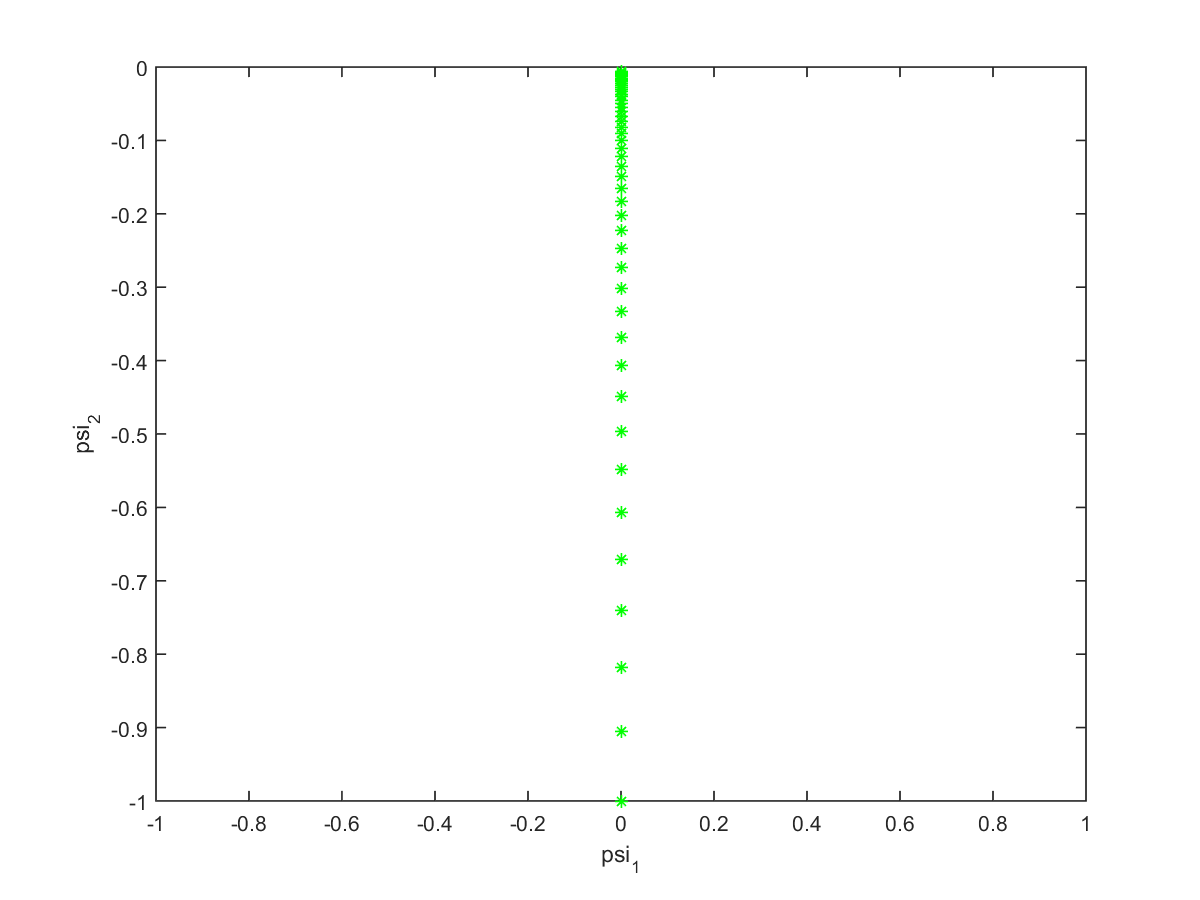
\includegraphics[width=0.5\textwidth]{psi_00.png}
\caption{$\psi_1 = 0$ в силу условий трансверсальности}
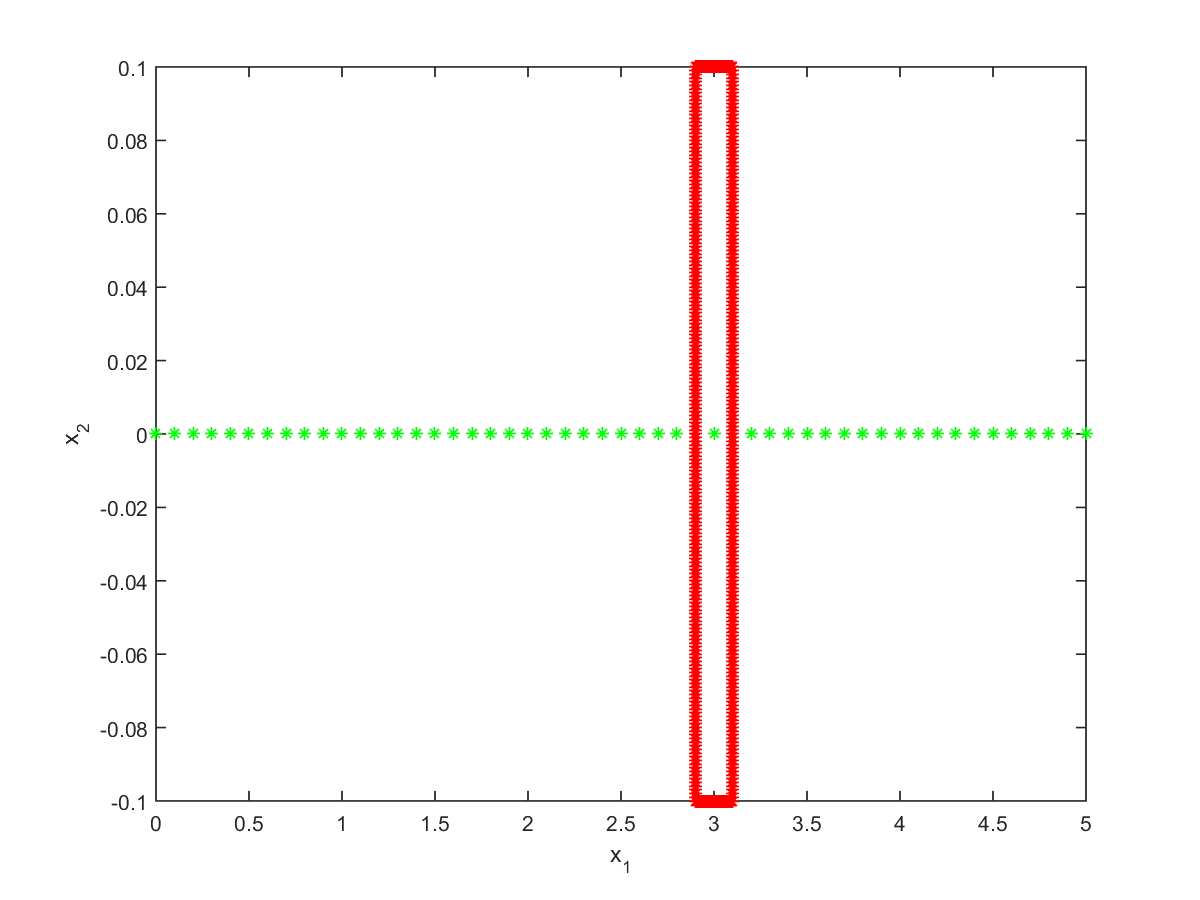
\includegraphics[width=0.5\textwidth]{psi_00x1x2.png}
\caption{Красным помечено множество достижимости. Видно, что за время $T$, траектория пролетает наше множество}
\end{center}
\end{figure}

\end{itemize}
\end{document}
